\section{Felhasználói Követelmények}

A felhasználónak mindenekelőtt be kell tudnia jelentkezni, ahhoz, hogy elérje a terméklistáját, ez azért fontos, mivel eszköz váltás esetén nem szeretnénk elveszíteni az addig követett termékeket. A bejelentkezéshez szükséges adatok a regisztrációkor megadott email cím, illetve jelszó. Mindezt az \ref{fig:login_activity_diag} ábra illusztrálja. A felhasználó jelszava base64 hash általi titkosítással van eltárolva, ezáltal az nem elérhető eredeti formájában, ezt a funkciót a bejelentkezést megvalósító Firebase Authentication valósítja meg, amely jelszó módosítási lehetőséget is lehetővé tesz.

\begin{figure}[h]
    \centering
    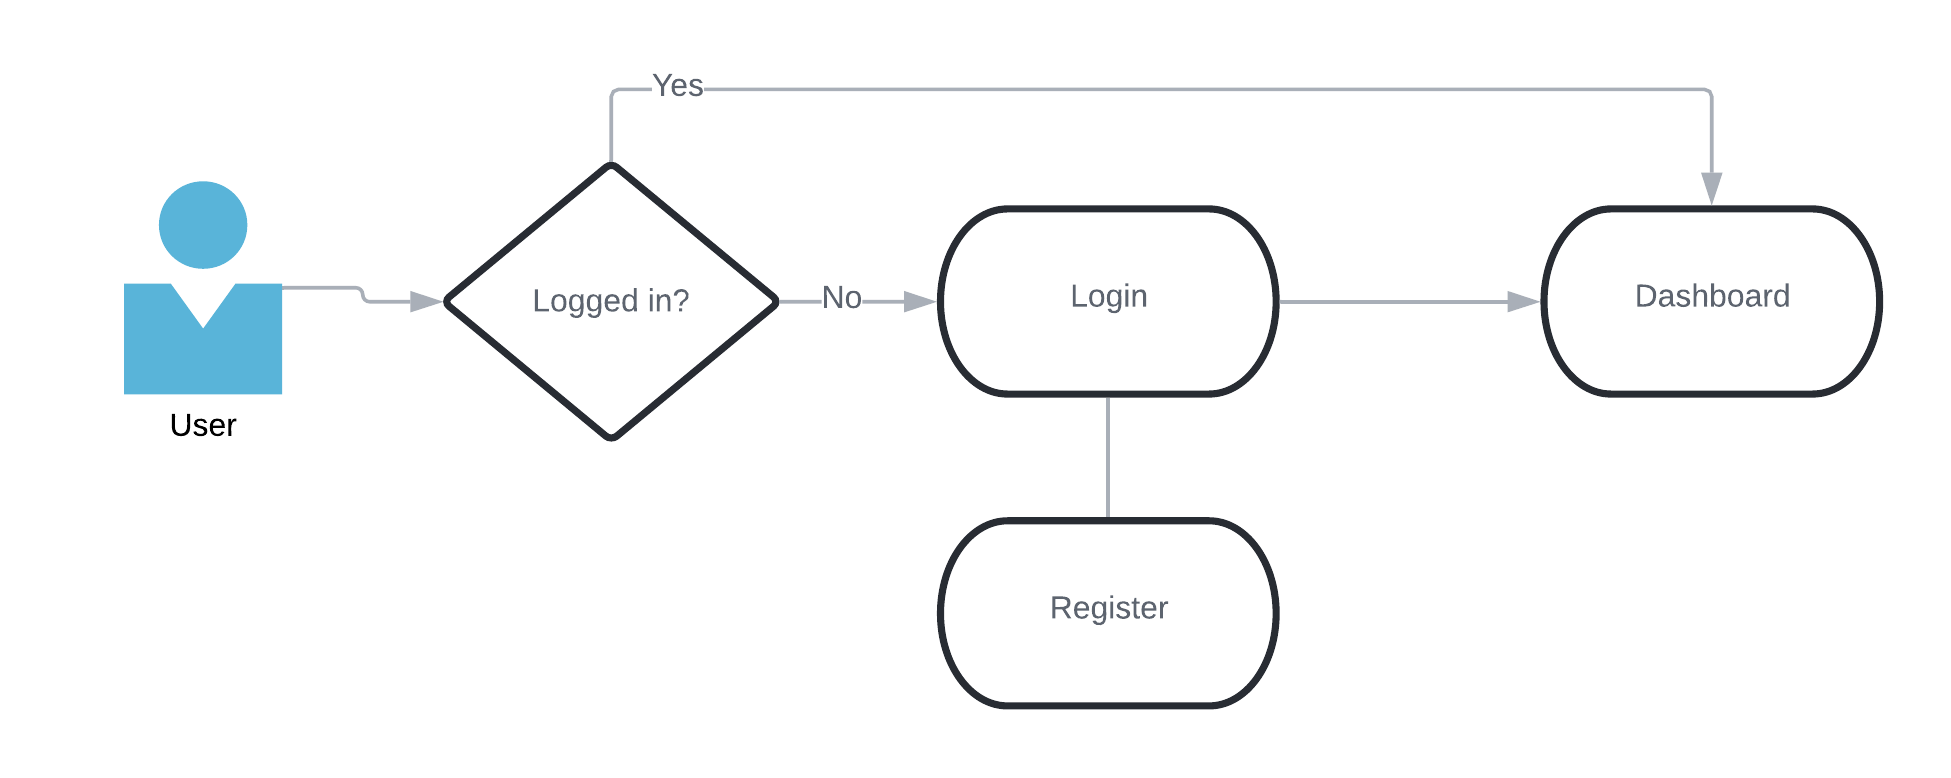
\includegraphics[scale=0.5, width=\textwidth]{figures/images/login_activity.png}
    \caption{Login Activity}
    \label{fig:login_activity_diag}
\end{figure}

Abban az esetben, ha a felhasználó nincs regisztrálva, megteheti ezt a „ Not registered? Click here! ” szövegre kattintva. A regisztrációhoz szükséges egy érvényes e-mail cím, valamint jelszó megadása. Sikeres regisztrálás esetén a felhasználó vissza kerül a bejelentkező ablakra, ahol be tud lépni, azzal a feltétellel, hogy az automatikusan küldött levél által visszaigazolta email címét.

A bejelentkezést követően a felhasználó a főoldalra kerül, ahol a követett termékek listáját tekintheti meg. A listában minden egyes elemnek látható a megnevezése, egy a terméket ábrázoló kép, illetve az adott termék aktuális ára. Továbbá ezen az oldalon lehetősége van a felhasználónak új termékeket hozzá adni a listához, lásd \ref{fig:dashboard_activity_diag} ábra.

\begin{figure}[H]
    \centering
    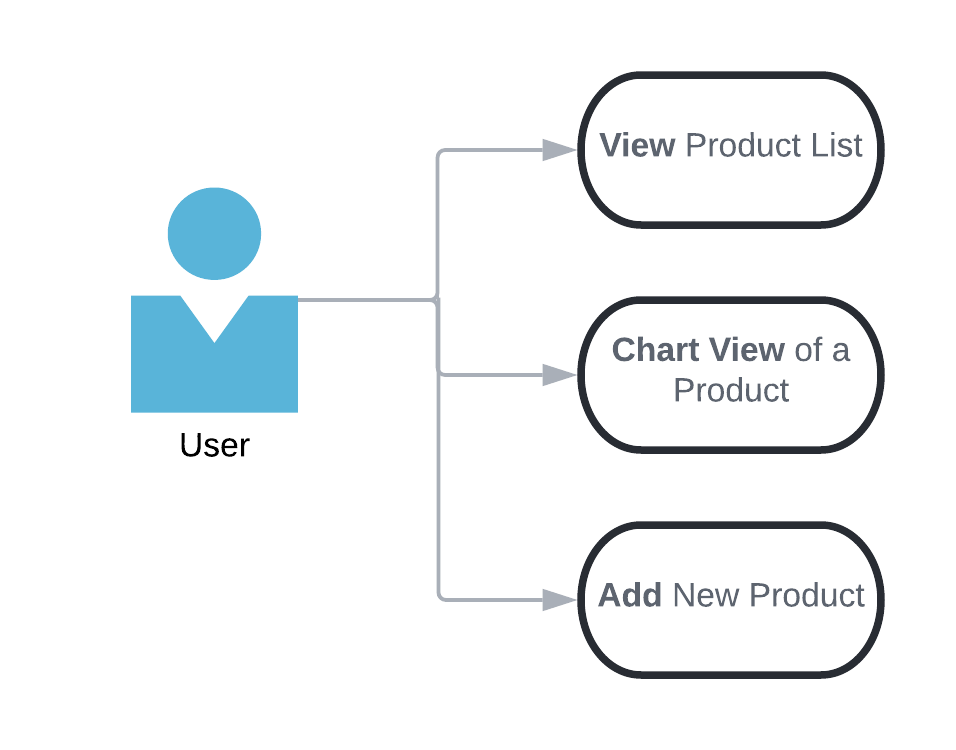
\includegraphics[scale=0.3]{figures/images/dashboard_activity.png}
    \caption{Dashboard Activity}
    \label{fig:dashboard_activity_diag}
\end{figure}

Egy a listában lévő elemre kattintva, az alkalmazás átvisz egy másik oldalra, ahol több információt kapunk a követett termékről. A termék árát tartalmazó gombra kattintva, egy grafikonon tekinthetjük meg a termék árának változását a hozzáadás napjától az aktuális dátumig, lásd \ref{fig:chart_example} ábra. Az „ See product page ” gombra kattintva az alkalmazás megnyitja a terméket tartalmazó weboldalt. Ugyanitt található a törlés gomb, melyre kattintva a termek törlésre kerül a listából és nem fogjuk tovább követni, lásd \ref{fig:detailed_view_diag} ábra.

\begin{figure}[H]
    \centering
    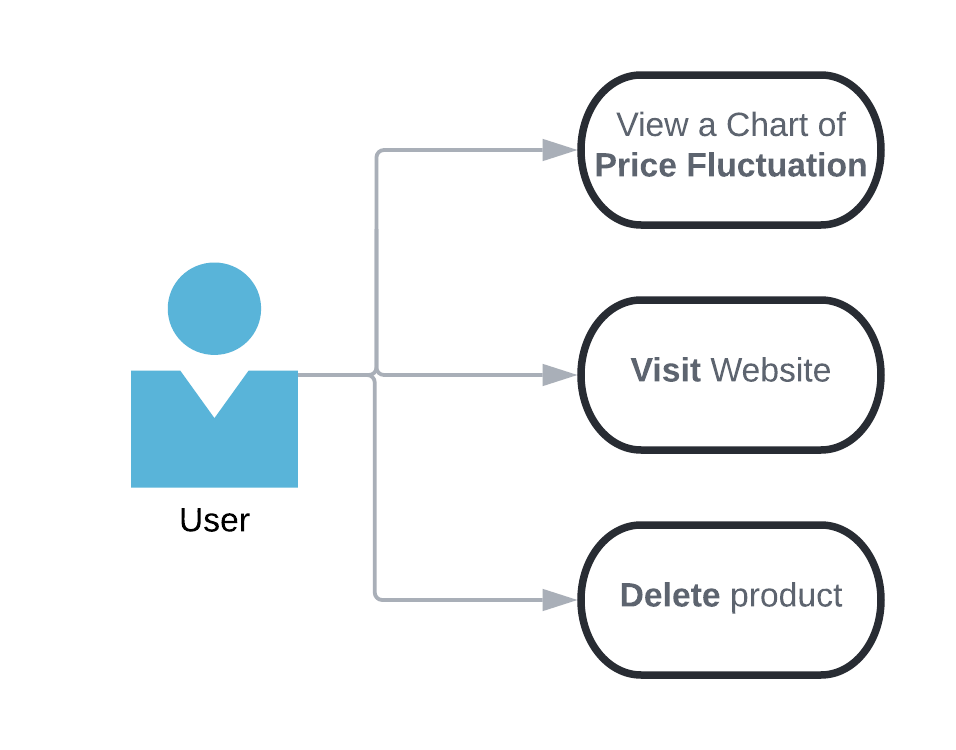
\includegraphics[scale=0.3]{figures/images/chart_view_activity.png}
    \caption{Detailed View}
    \label{fig:detailed_view_diag}
\end{figure}

\begin{figure}[H]
    \centering
    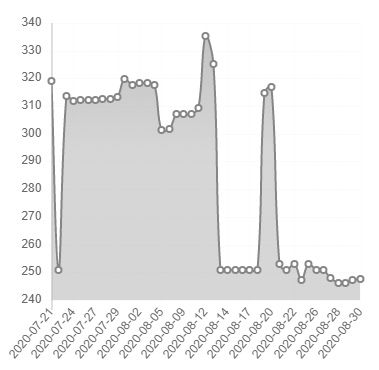
\includegraphics[scale=1]{figures/images/chart_example.png}
    \caption{Chart of Price Change}
    \label{fig:chart_example}
\end{figure}

A felhasználó rendelkezésére áll továbbá két menü. Egy információs, amely röviden leírja az alkalmazás használatát, illetve tartalmazza az általa támogatott weboldalak listáját. A másik a felhasználó fiókjával kapcsolatos információkat és funkciókat tartalmaz. Itt tekintheti meg a felhasználó, hogy milyen email címmel jelentkezett be, megváltoztathatja az aktuális jelszavát, törölheti a fiókját, illetve kijelentkezhet az alkalmazásból, lásd \ref{fig:additional_info} ábra.

\begin{figure}[H]
    \centering
    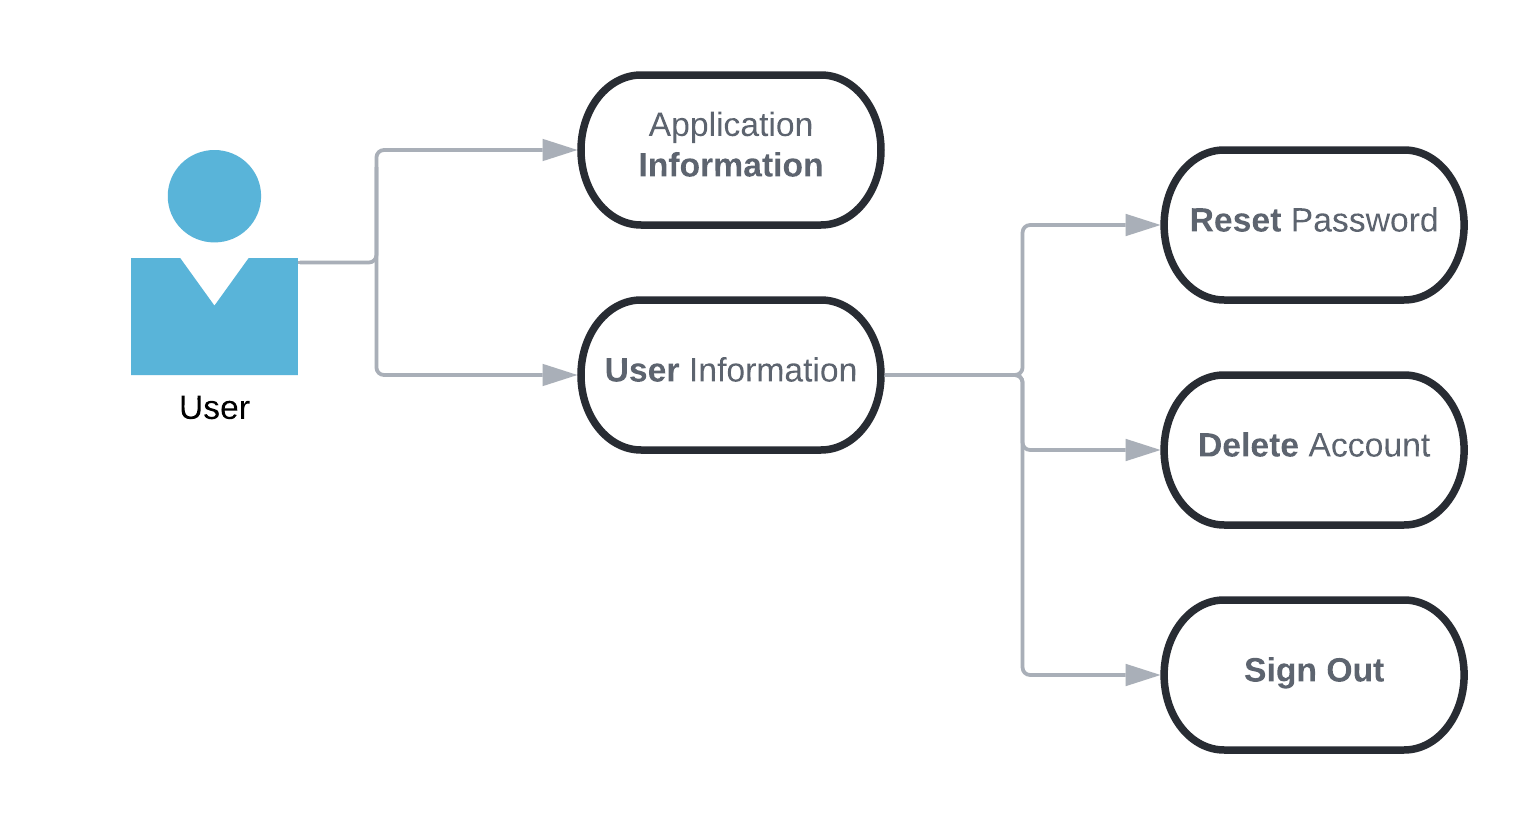
\includegraphics[scale=0.3]{figures/images/additional_features.png}
    \caption{Additional information}
    \label{fig:additional_info}
\end{figure}

\section{Rendszer Követelmények}

\subsection{Funkcionális követelmények}

A rendszernek mindenek elött, egy bejelentkezési, illetve, regisztrálási felülettel kell rendelkeznie. Regisztrálás után, a felhasználónak egy ellenőrző email-t kell kapnia, amivel igazolja, hogy ő a cím tulajdonosa. A bejelentkezés nem lehetséges, abban az esetben, ha a felhasználó nem igazolta vissza az előbb említett email-ben a címét. A cím igazolása egy linkre való kattintással történik.

A felhasználónak lehetősége van a jelszavának módosítására melyet a bejelentkezési felületről ér el. Miután a felhasználó beírta az email címét, egy levelet fog kapni az adott címre, amelyen keresztül új jelszót tud beállítani.

Bejelentkezést követően, a felhasználó egy felületet lát, melyen bizonyos műveleteket végezhet. Megtekintheti a profiljához tartozó email címét, valamint törölheti a felhasználóját. Ugyanakkor, lehetősége van kijelentkezni az alkalmazásából melynek hatására újra a bejelentkezési oldalra kerül.

Ugyancsak a főoldalról a felhasználónak lehetősége van az alkalmazás használatával kapcsolatos információk megtekintésére mely tartalmaz egy listát is. A lista bizonyos weboldalkát tartalmaz, melyeket kiválasztva, az alkalmazás átirányít az adott elem oldalára.

A felhasználónak lehetősége van termékeket hozzáadni és kitörölni a listájából, valamint görgetni a lista tartalmában. A terméklistában egy elemet kiválasztva, részletes reprezentációt kap az adott elem tárolt adatairól.

\textcolor{red}{a rendszer magatol kell erzekelje ha az adatbazisban valtozas tortent ?ez ide johet?}

\subsection{Nem-Funkcionális követelmények}

A rendszer backend része, mely a felhasználok által hozzáadott teremkék árainak ellenőrzését, frissítését, hozzáadását végzi, megszakítás nélkül kell működnie, napszaktól függetlenül. A rendszernek képesnek kell lennie Python 3-as kódot futtatnia, fel kell legyen telepítve a Python 3.8.0. Létfontosságú, hogy egy stabil internetkapcsolattal rendelkezzen, vagyis a kapcsolatban ne legyenek megszakítások, valamint a fel-letöltési sebesség ne csökkenjen 10 Mb/s alá, annak érdekében, hogy megfelelő sebességgel lehessen az adatfeldolgozást, valamint az adatok adatbázisba való fel-, letolteset elvégezni. Amennyiben a kapcsolat megszakad, a rendszer azonnal próbáljon újrakapcsolódni, mindaddig amig ez a művelet nem sikers.

% TODO
\textcolor{red}{TODO: chromium alapu bongeszokon kell fusson, internet kapcsolat} \newline
\textcolor{red}{UPDATE: megirtam hogy elvaras hogy chrome alapon fusson es milyen verzio, ez eleg?}

A rendszer vizuális felülete két alapvető platformon kell elérhető legyen. Az egyik egy böngésző kiegészítő, mely bármilyen Chromium alapú böngészőre telepíthető, asztali, valamint hordozható számítógépek eseteben is, legalább 58-as verziójú Chrome-ot tamogatva. Természetesen ebben az esetben is elengedhetetlen az internethez való csatlakozás.

%TODO
\textcolor{red}{TODO: android operacios rendszeren, min x.x verzio, internet kapcsolat} \newline
\textcolor{red}{UPDATE: megirtam androidos reszre is hogy mi a kovetelmeny}

A másik egy telefonos alkalmazás, mely Android operációs rendszerrel felszerelt készülékeken legyen elérhető. Az alkalmazásnak legalább 7.0 verziójú Androiddal felszerelt telefonokon kell működnie, mely rendelkezik stabil internetkapcsolattal.
\textcolor{red}{Q: Ide jonnek azok az informaciok, hogy telefonon legyen dark mode pl, listaban jelenitsuk meg a tarmekeket stb? kinezettel kapcsolatos kovetelmenyek}


A rendszer a Firebase által biztosított Realtime Database nevű adatbázist kell használnia az adatok tárolására. A felhasználó bejelentkezését és a fiókjához tartozó műveleteket szinten a Firebase által biztosított Authentication szolgáltatás végezze, mivel ez biztonságos módon tárolja a szükséges információkat, ugyanakkor, a jelszavakat titkosítva kezeli. Továbbá, ezen keresztül lehessen új jelszót beállítani, a felhasználót törölni, ugyanakkor a regisztrálás után szükséges email visszaigazolása is ezen a szolgáltatáson keresztül történjen, mivel ezekre egyszerűen használható, ugyanakkor hatékony és biztonságos megoldást nyújt.

Az alkalmazás könnyen használható kell legyen, a felhasználónak minden funkciót három kattintáson belül el kell érnie. 

Amikor a felhasználó egy új terméket szeretne hozzáadni a listájához, ne keljen több mint 5 másodpercet várnia ahhoz, hogy az új termék megjelenjen a listájában. 
